\section{Решения задач}
Опишем возможные способы решения задачи $pred$
и $topN$ в нечеткой модели при применении правила вывода
$\Pi_f$ (\ref{my-pi}).
Приведенные способы не являются единственно возможными способами решения.

\subsection{Решение задачи $topN$}
Задача $topN$ может быть решена с помощью линейного поиска
таких объектов, что $u_a \R i$.


На рисунке <<Блок-схема алгоритма решения задачи $topN$ в нечеткой модели при
	использовании $\Pi_f$>> (\ref{dia:fuz-topn}) изображена блок-схема алгоритма
решения задачи $topN$ в нечеткой модели при использовании
правила вывода $\Pi_f$.
\begin{figure}[hbtp]
	\caption{Блок-схема алгоритма решения задачи $topN$ в нечеткой модели при
	использовании $\Pi_f$}
\begin{center}
	\label{dia:fuz-topn}
 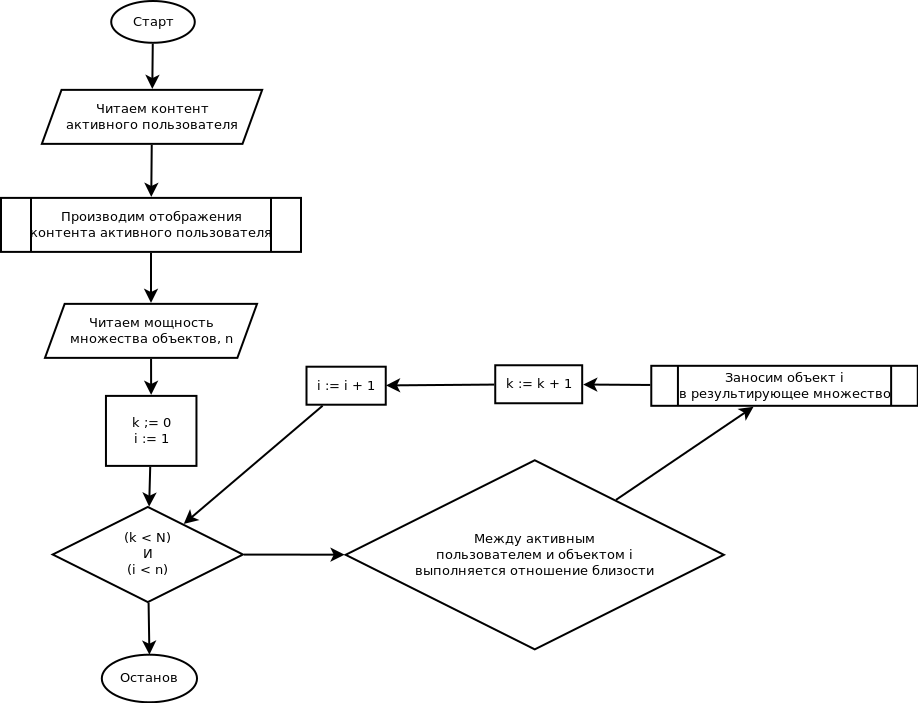
\includegraphics[width=7in,height=8in]{pics/algs/fuz-topn.png}
\end{center}
\end{figure}
Блок-схеме (\ref{dia:fuz-topn}) соответствует псевдокод, представленный на
изображении <<Алгоритм решения задачи $topN$ при использовании правила
	вывода нечеткой модели>> (\ref{alg:fuz-topn}).

\begin{figure}[htb]
	\caption{Алгоритм решения задачи $topN$ при использовании правила
	вывода нечеткой модели}
	\label{alg:fuz-topn}
	%\begin{algorithm}
		\begin{algorithmic}[1]
			\State $n \gets 1$
			\State $I_{topN} \gets \varnothing$
			\For {$i \gets 1 \to |I|$}
			\If{$\rh(u_a, i) \ge \Delta_{\R}$}
			\State $I_{topN} \gets I_{topN} \bigcup \{ i \}$
			\State $n \gets n + 1$
			\EndIf
			\If{$n = N$}
			\State Стоп
			\EndIf
			\EndFor
		\end{algorithmic}
	%\end{algorithm}
\end{figure}

\subsection{Свойства решения задачи $topN$}
\begin{trm}
	\label{pif_acc}
	Если $\Pi_f$ определено разработчиками так, что $\forall$ $(u_a, i, \rho(u_a, i)) \in P$
	$|\rho(u_a, i) - \rh(u_a, i)| = 0$, то эффективность решения
	по критерию качества гарантированна.
\end{trm}

Результирующее множество имеет вид $\{(u_a, i, \rh(u_a, i)): \rh(u_a, i) \ge
\Delta_{\R}\}$. Так как $|\rho(u_a, i) - \rh(u_a, i)| = 0$, поэтому
$\rh(u_a, i) \ge \Delta_{\R}$, а, значит, $u_a \R i$ и решение эффективно по
$\eat$, что и требуется по задаче.

Таким образом, получаем, что
\begin{trm}
	\label{fuz-cond-topn}
достаточным условием эффективности решения задачи $topN$ по критерию качества является
такое задание $\Pi_f$, что
$|\rh(u_a, i) - \rho(u_a, i)| = 0$
\end{trm}

Асимптотическая сложность решения задачи $topN$ равна $O(|I|)$.

\subsection{Решение задачи прогнозирования}
Правило вывода нечеткой модели (\ref{my-pi}) заключается в реализации функции $\rh$.
Поэтому прямое решение задачи прогнозирования, без применения каких-либо
алгоритмов, заключается только в расчете значения $\rh(u_a, i_{\bot})$.


На рисунке <<Блок-схема алгоритма решения задачи прогнозирования в нечеткой модели при
	использовании $\Pi_f$>> (\ref{dia:fuz-p}) изображена блок-схема алгоритма
решения задачи прогнозирования  в нечеткой модели при использовании
правила вывода $\Pi_f$.
\begin{figure}[hbtp]
	\caption{Блок-схема алгоритма решения задачи прогнозирования в нечеткой модели при
	использовании $\Pi_f$}
\begin{center}
	\label{dia:fuz-p}
 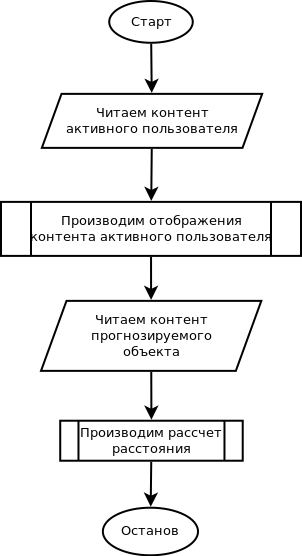
\includegraphics[width=4in,height=5in]{pics/algs/fuz-p.png}
\end{center}
\end{figure}
Блок-схеме (\ref{dia:fuz-p}) соответствует псевдокод, представленный на
изображении <<Алгоритм решения задачи прогнозирования при использовании правила
	вывода нечеткой модели>> (\ref{alg:fuz-p}).

\begin{figure}[htb]
	\caption{Алгоритм решения задачи прогнозирования при использовании правила
	вывода нечеткой модели}
	\label{alg:fuz-p}
	%\begin{algorithm}
		\begin{algorithmic}[1]
			\State $\rh(u_a, i_{\bot})$ \Comment{Нужно провести только расчет
			прогнозной функции}
		\end{algorithmic}
	%\end{algorithm}
\end{figure}

%\begin{figure}[h]
%\caption{Решение задачи прогнозирования}
%\begin{algorithm}\label{mysolve-p}
%\begin{algorithmic}[1]
%\State $\delta(u_a, i_{\bot}) \gets 1 - \rh(u_a, i_{\bot})$
%\end{algorithmic}
%\end{algorithm}
%\end{figure}

\subsection{Свойства решения задачи прогнозирования}

\begin{trm}
	\label{pif_acc_pred}
	Если $\Pi_f$ определено разработчиками так, что $\forall$ $(u_a, i, \rho(u_a, i)) \in P$
	$|\rho(u_a, i) - \rh(u_a, i)| \le \varepsilon_p$, то эффективность решения
	по критерию качества гарантированна.
\end{trm}

Эффективность решения задачи $pred$ зависит от
аккуратности задания $\Pi_f$.
Если функция $\rh$ реализована так, что
$|\rh(u_a, i) - \rho(u_a, i)| \le \varepsilon_p$, то решение будет эффективным,
что следует из способа решения задачи.

Таким образом, получаем, что
\begin{trm}
	\label{fuz-cond-pred}
достаточным условием эффективности решений по критерию качества является
такое задание $\Pi_f$, что
$|\rh(u_a, i) - \rho(u_a, i)| \le \varepsilon_p$
\end{trm}

Асимптотическая сложность решения задачи $pred$ равна $O(C)$.
%\subsection{Интерполяционное решение задачи прогнозирования}
%
%\subsection{Свойства интерполяционного решения задачи прогнозирования}




